\newpage
\subsection{The Query Model}\label{section:queryModel}

\textcolor{gray}{
\begin{itemize}
    \item General formalization: Continuous queries.
    \item Fraud patterns identified - Definition and their formalizations
    \item Profundizar más en el que se ha probado. Describir implementación.
\end{itemize}
}
\fmc{Recabar enlaces de definiciones de fraudes bancarios pasados por whats}

\subsubsection*{The Query Model: Continuous Query Model}
\fmc{Formalización del query model. Completar más.}
In the context of our application, taking into account that the input data of our system takes the form of a continuous data stream, we categorize our query model under the \emph{continuous query} model \cite{CQ-babu2001continuous, CQ-zaniolo2012logical}. The continuous query model is the ideal query model for applications considering queries evaluated over data streams (unbounded sequences of timestamped data items), in contrast with classical query evaluation processes, where the data to query is stable, with small or infrequent updates. 

Although, part of the data source of our application is stable (the stable bank database), the input of our system consists of a data stream, data in motion and continuously changing, as it is the ATM transactions input data stream. 

In our work, we tackled the problem of evaluating continuous queries corresponding to anomalous patterns of ATM transactions against a continuously evolving PG representing a bank database. 
The bank database is continuously evolving due to the input ATM transactions data stream that is continuously receiving.
The anomalous patterns of ATM transactions are identified in the volatile (PG) subgraph of the considered database. With this, a query on our PG database can be defined as a PG graph pattern with constraints over some of its properties. Evaluating such a query consists on identify if there is a subgraph of the database that matches the given graph pattern and satisfies its constraints.

\subsubsection*{The Query Model: Fraud Patterns Definition}

It is not trivial to establish what is and in which circumstances an ATM transaction can be considered anomalous. Based on a work that have addressed this characterization \cite{FP-magdalena2021artificial} we intend to find a proper characterization and then define the graph patterns associated to these anomalies. The exact topology of an anomaly will depend on its own nature. Moreover, definition of patterns can be beyond ATM transactions by considering online card transactions. In what follows, we propose a characterization of some possible anomalous patterns of ATM transactions and the definition of their associated PG graph patterns. 

\begin{enumerate}
\renewcommand{\labelenumi}{\Roman{enumi}.} % Roman numerals for the list
    \item Card cloning characterization
    \item Lost-and-stolen card characterization
    %\item Anomalous amount of withdrawals in a time period
    \item Other possible fraud scenarios
\end{enumerate}


\paragraph{I - Card Cloning Characterization\\\\}

\textcolor{gray}{Definition references:
\begin{itemize}
    \item \cite{FP-unit21_card_cloning}
    \item 
\end{itemize}
}

\emph{Card cloning} can be defined as a ``type of fraud in which information on a card used for a transaction is covertly and illegally duplicated. Basically, it’s a process thieves use to copy the information on a transaction card without stealing the physical card itself. This information is then copied onto a new or reformatted card, allowing criminals to use it to make fraudulent purchases or gain unauthorized access to a person’s accounts.```\cite{FP-unit21_card_cloning}.

There are many possible ways to detect a card cloning scenario, among others the analysis of the customer's transaction data to construct typical transaction behaviors so to be able to detect uncommon transaction behaviors. However, in our work we propose an alternative possible method based on a PG graph pattern detection.

In particular, the method consists on detecting card-ATM activity of the same card at different ATMs taking place within an unfeasible time distance difference. That is, when at a certain time a transaction is made in an ATM and after that, another transaction is started with that same card in a different ATM location such that the distance between the two ATM locations is impossible to cover in the time difference between the two transactions. The detection of this anomalous scenario is represented on the PG graph pattern of the Figure \ref{img:graphPattern-1}. 

\begin{figure}[H]
  \centering
  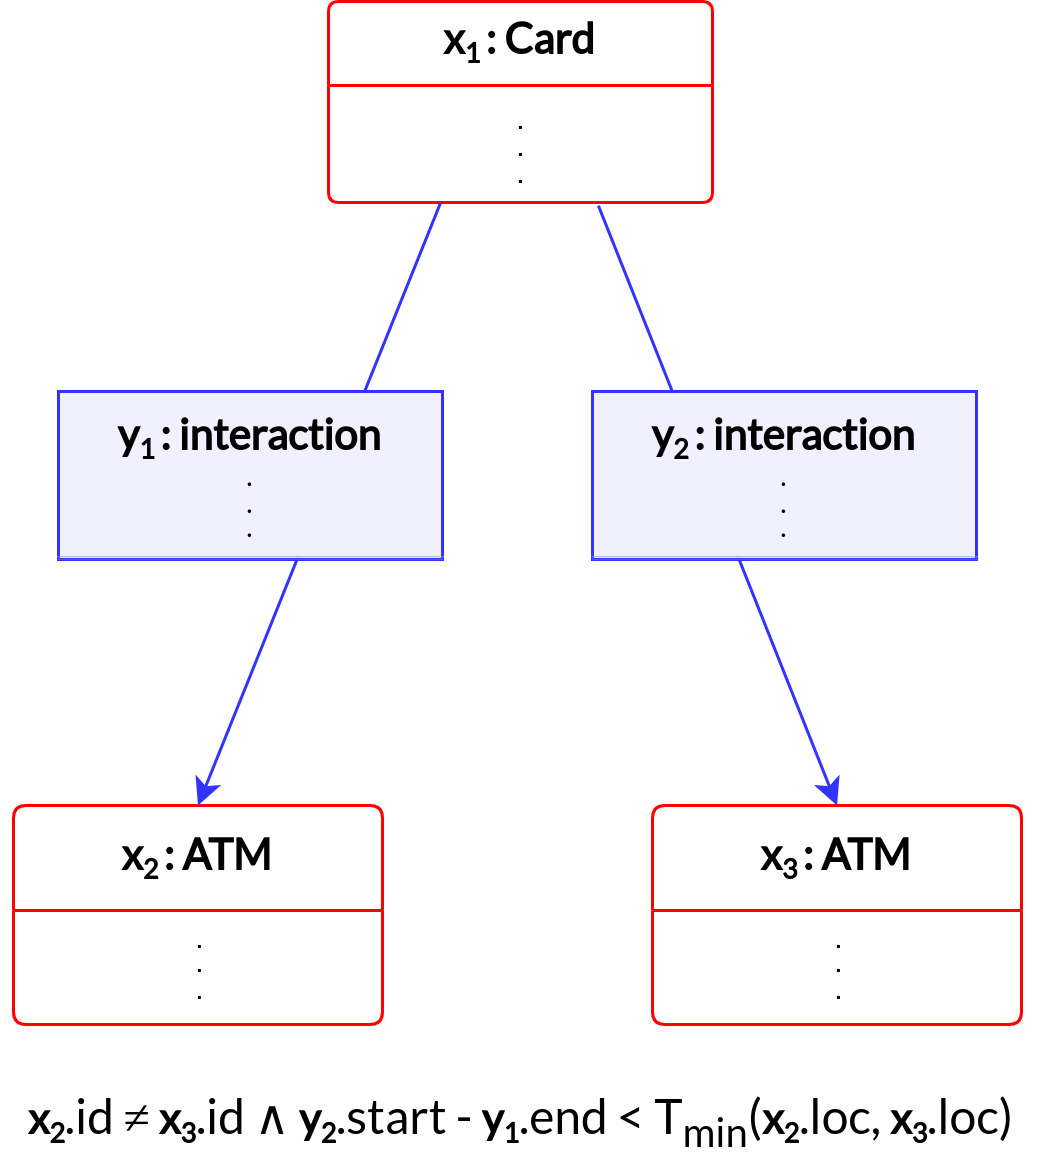
\includegraphics[scale = 0.8]{images/2-QueryModel/graphPattern-1.png}
  \caption{Card Cloning Characterization - Graph Pattern}
  \label{img:graphPattern-1}
\end{figure}

The pattern consists on Card entity $x_1$, having two interaction relations $y_1$ and $y_2$ with two different ATMs $x_2$ and $x_3$, respectively, such that the time difference between the ending time of the first interaction $y_1.\textit{end}$ and the starting time of the second interaction $y_2.\textit{start}$, is not sufficient to cover the minimum time needed to travel from the first to the second ATM location $T_{min}(x_2.\textit{location}, x_3.\textit{location})$. As a whole:

$$
\small
x2.id \ne x3.id \ \land \ y_2.\textit{start} - y_1.\textit{end} < T_{min}(x_2.\textit{location}, x_3.\textit{location})
$$

where $x_2.\textit{location}$ location represents the location coordinates pair of the $x_2$ ATM: $x_2.location = (x_2.loc\_latitude, x_2.loc\_longitude)$. Same for the $x_3$ ATM.

\fmc{TODO: Poner qué es / cómo se calcula el tmin (la formula, que es parametrizable en base a la velocidad max decidida...}

An example of this kind of anomalous card-ATM interaction, could be one as represented on Figure \ref{img:graphPattern-1-Example}, in which an ATM interaction with a certain card is finished at time 22:14 in Barcelona, and then another interaction with that same card starts at time 22:56 of that same day in Madrid. Clearly this should be reported as this kind of anomalous scenario since it is impossible, for the time being, to cover the distance between these two cities in that time difference.

\begin{figure}[H]
  \centering
  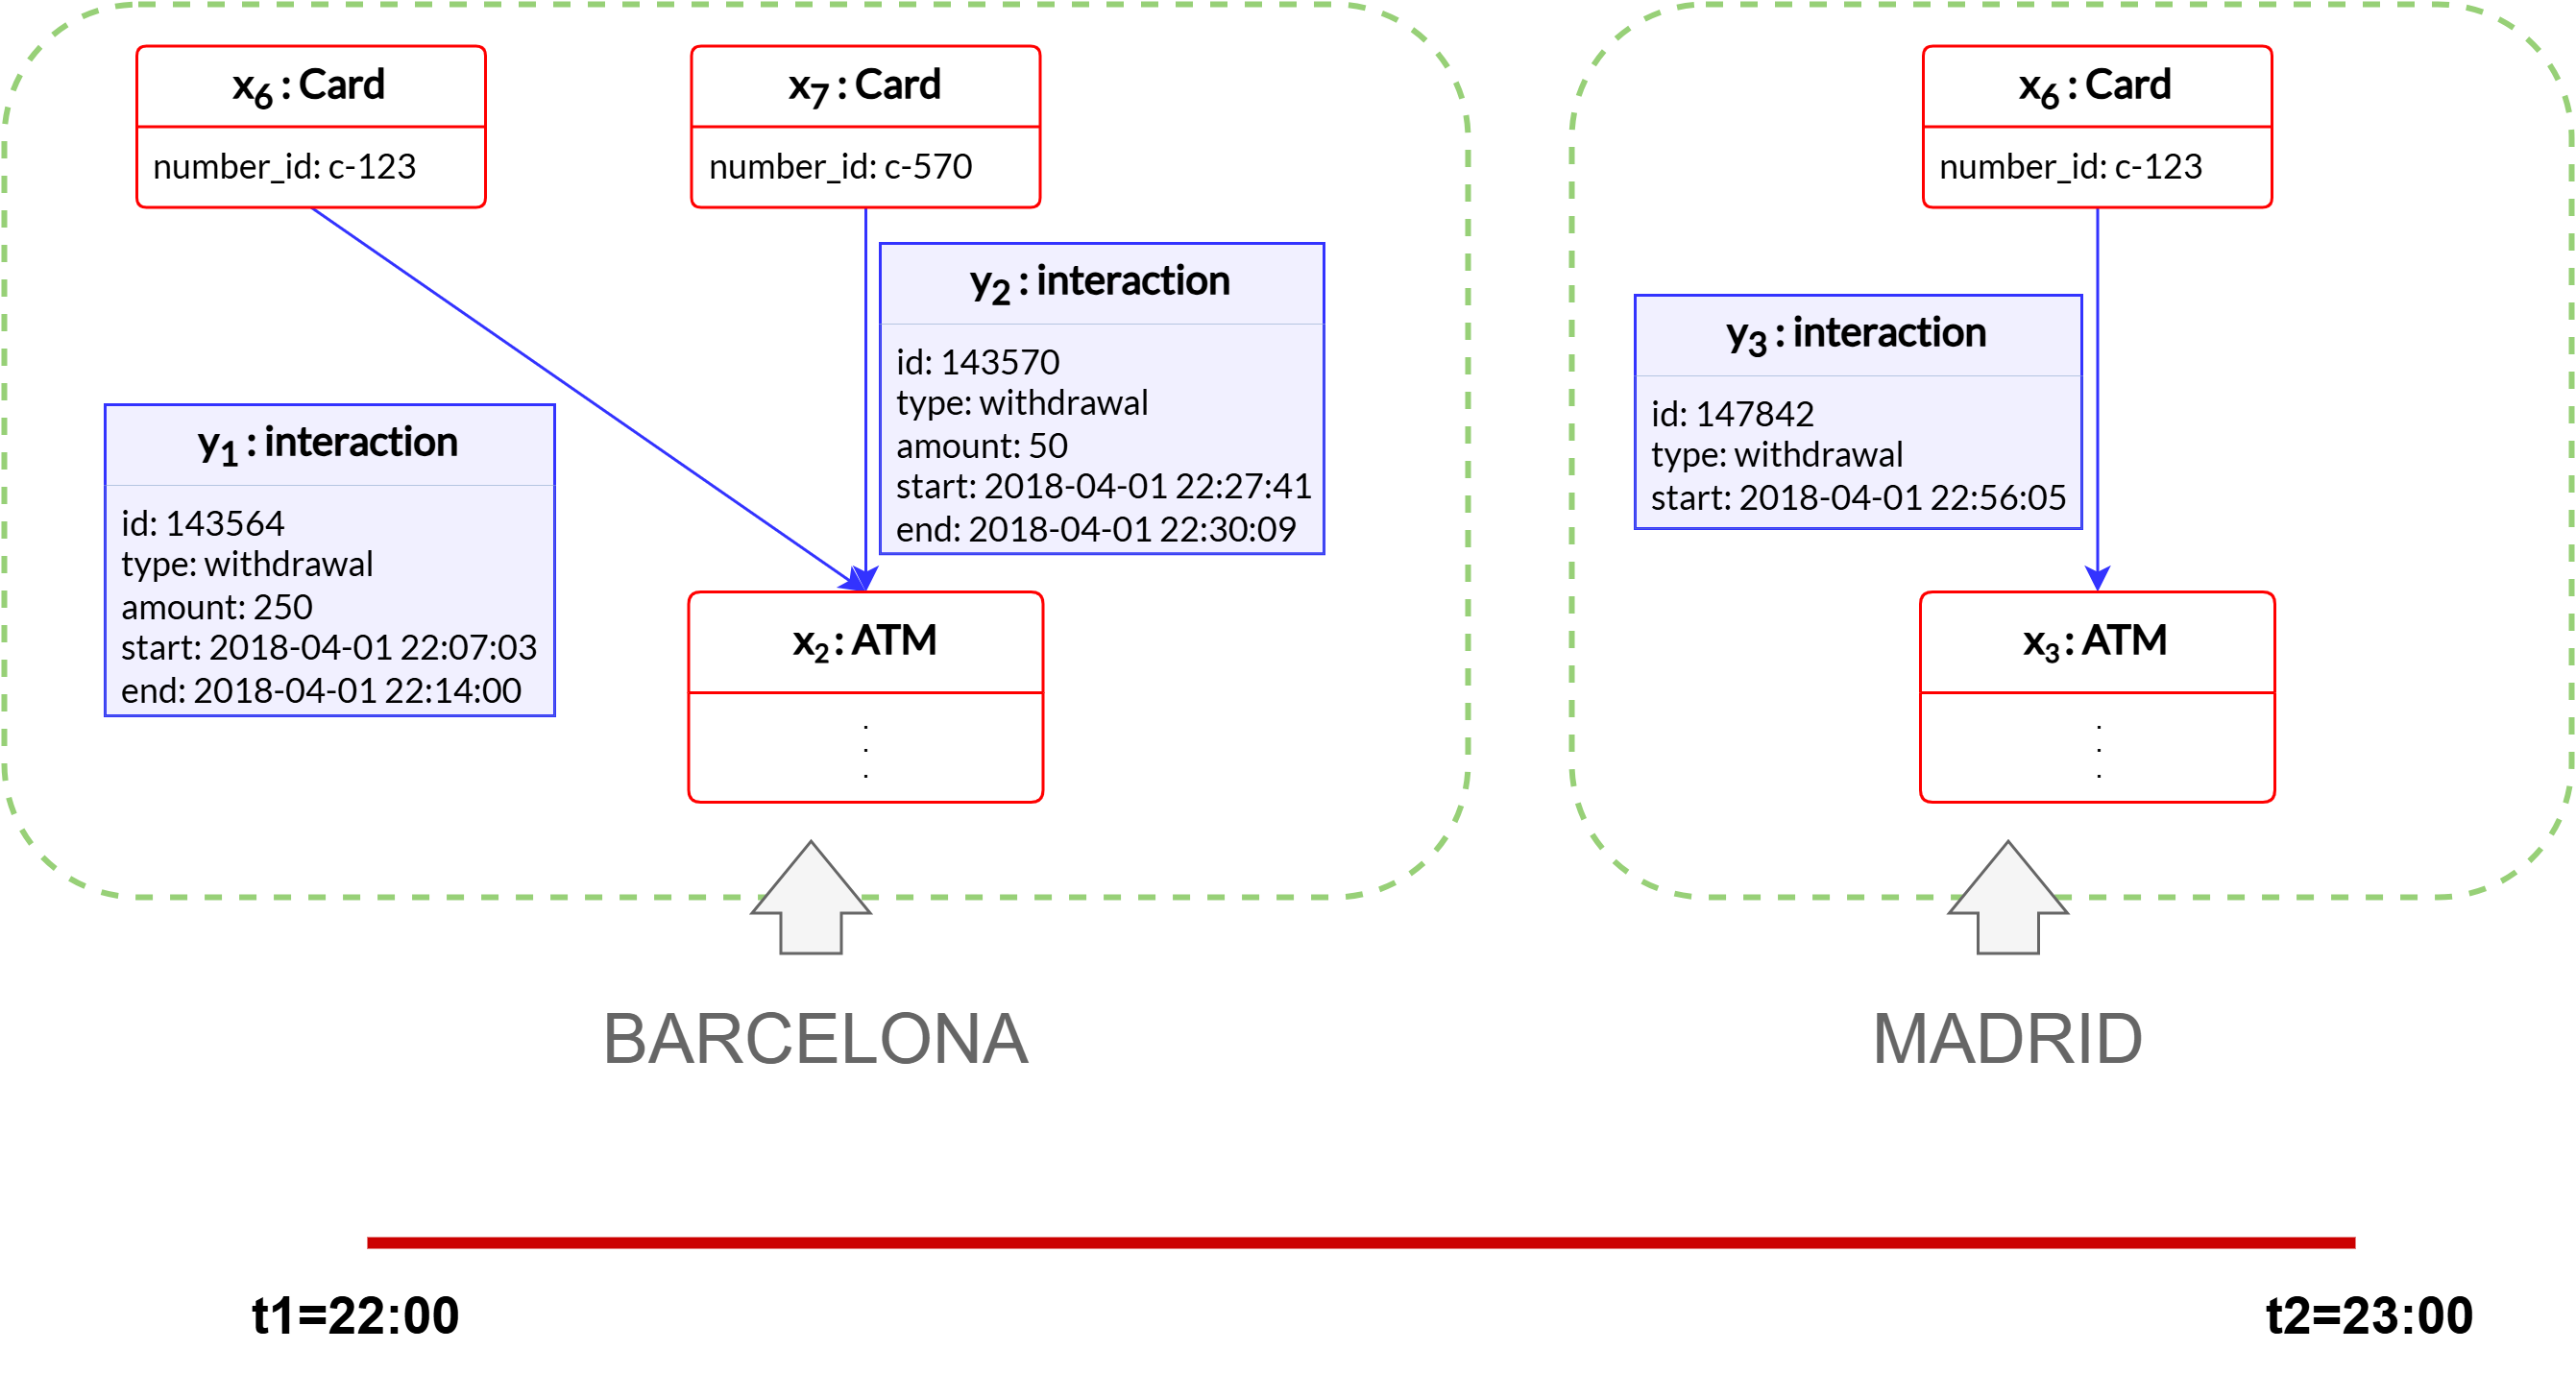
\includegraphics[scale = 0.7]{images/2-QueryModel/FP1-Example.png}
  \caption{Card Cloning Characterization - Example}
  \label{img:graphPattern-1-Example}
\end{figure}

\paragraph{II - Lost-and-Stolen Card Characterization\\\\}

\fmc{Referencias para este tipo de anomalía. Definir mejor... Completar}
\textcolor{gray}{Definition references:
\begin{itemize}
    \item https://www.datavisor.com/wiki/lost-or-stolen-card-fraud/
    \item https://www.americanexpress.com.kw/en-kw/fraud-protection-center/lost-and-stolen-card-fraud/
\end{itemize}
}

"Lost-and-stolen card is the fraud scenario produced when a card is physically stolen or is lost, and is then used by a criminal, posing as you, to obtain goods and services" \cite{FP-lost-and-stolen-americanexpress2025}.

A possible way that we propose to detect this kind of scenario is through the tracking of a typical behavior that it is produced when the card is used by the criminal. That is, when obtained, the fraudster tries to do as many as possible money withdrawals in different ATMs before the owner of the card realises and asks the bank to freeze the card. The detection of this kind of fraud scenario is modeled with a PG graph pattern as the one represented on Figure \ref{img:graphPattern-2}.
\fmc{DUDA: Indicar en el dibujo que el tipo de interacción/operación es el de withdrawal?}

\begin{figure}[H]
  \centering
  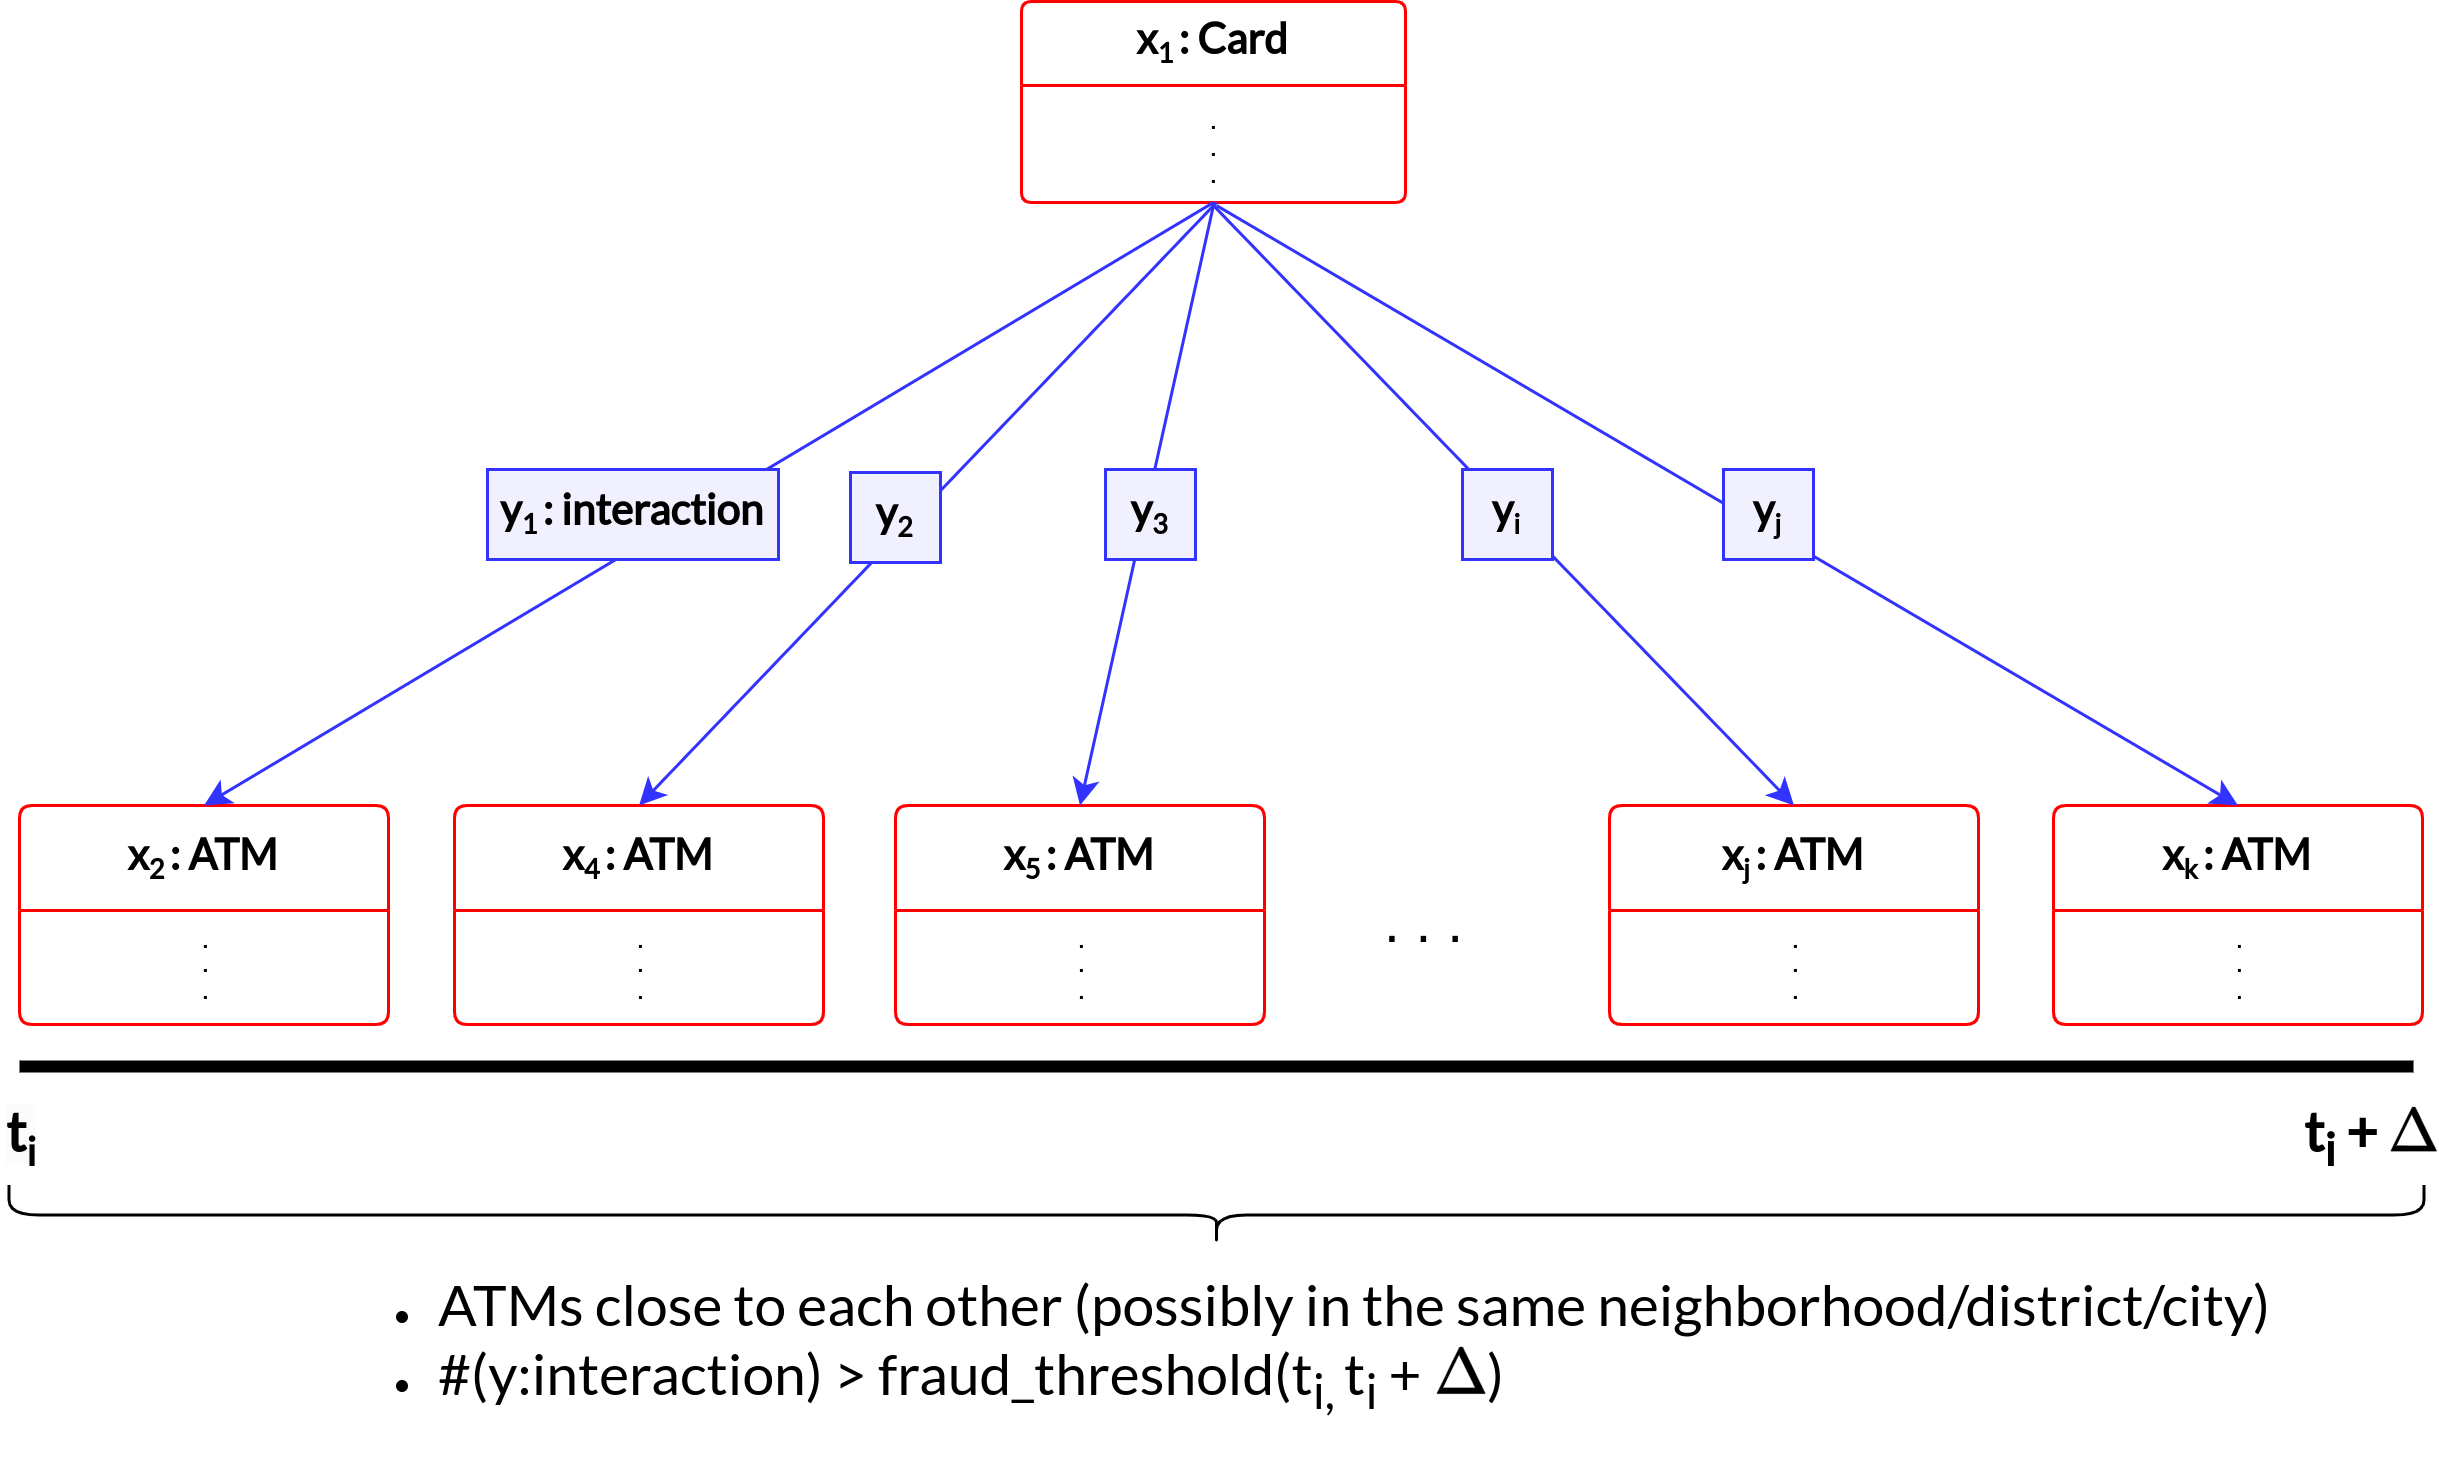
\includegraphics[scale = 0.7]{images/2-QueryModel/graphPattern-2.png}
  \caption{Lost-and-Stolen Card Characterization - Graph Pattern}
  \label{img:graphPattern-2}
\end{figure}

On it we define a Card entity $x_1$ having a number $k$ of interactions $y$ at different ATMs $x_2 ... x_k$ within a time interval $[t_i, t_i + \Delta]$, where $t_i = y_1.\textit{start}$ and $t_i + \Delta = y_k.\textit{start}$, such that $k$ is considered to be an usual high number of withdrawals for that time interval. A reference for the usual number of withdrawals on a certain time interval for a specific cardholder can be obtained from the gathered cardholder behavior \emph{withdrawal\_day} card entity property.
Another indicator of this scenario to be considered could also be the \emph{amount} value of the withdrawal operations performed, which is normally a low value to prevent that the card owner realises.

\fmc{Otro tipo de fraude que comentamos es el de detectar más de una extracción en un tiempo dado... realmente creo que quedaría dentro de este mismo tipo de fraude.}

%\paragraph{III - Anomalous Amount of Withdrawals Within a Time Period\\\\}
\paragraph{III - Other possible fraud scenarios\\\\}

Some other anomalous scenarios for which more graph patterns could be defined are:
\begin{itemize}
    \item \textbf{Anomalous location usage}: When a transaction is made in a location out of the threshold distance of the usual/registered address of the cardholder.
    \item \textbf{Anomalous number of operations}: Related with the II pattern characterized, we could also define a graph pattern related with a higher than average number of operations of any kind (withdrawal, inquiry, transfer or deposit) for a cardholder in a certain time interval.
    \item \textbf{Anomalous high expenses:} Similar to the II pattern, but in this case, not considering only the number of the withdrawal operations performed on a certain time interval, but the amount of the withdrawal operations on a certain time interval. This could indicate an anomalous behavior of the cardholder, withdrawing an amount of money way higher for a considered time interval.
\end{itemize}


\subsubsection*{The Query Model: Fraud Patterns Algorithmic Description}

So far, among all the characterized anomalous scenarios as PG graph patterns, for our proof of concept, we implemented the detection of the first defined graph pattern, the graph pattern related with the card cloning characterization.

\fmc{En lo que sigue se explica:\\
1. el algoritmo de inicio en el que se tenía un subgrafo de todas las interacciones que llegaban por cada una de las cards. Se hacía el check de una interacción entrante con cada una de las interacciones del subgrafo. 
\\ 2. Como se vio que se podía simplificar (bastaba con hacer el check con la más reciente del subgrafo, se simplificó el subgrafo (almacenando solo la interaccion más reciente) y también el algoritmo...\\
DUDA: Pongo directamente el modelo/forma final o dejo todo?}

\ad{Yo pondría el final pero si te gusta más que esté todo, déjalo todo.}

\fmc{Esta parte creo que sería más conveniente explicarla en el apartado de Implementation del \DPATM porque ahi ya se han explicado los subgrafos, los filter stages... y otros conceptos necesarios... REORDENAR}
\paragraph{I - Card Cloning Graph Pattern Algorithm\\\\}
\fmc{Faltaría explicar que se tiene un subgrafo por cada card donde se van acumulando/almacenando todas las relaciones/interacciones de la card...}
A first algorithmic proposal to detect this kind of fraud pattern is the one shown in the algorithm
\ref{alg:check-fraud-1}. Note that $S$ refers to the filter's subgraph and $e_{new}$ is the new incoming edge belonging to the filter, such that it is a opening interaction edge, since in the case it is a closing interaction edge, we do not perform any fraud checking operation \text{CheckFraud()}.

\begin{algorithm}[H]
    \small
    \begin{algorithmic}[1]
    \REQUIRE $S$ is the subgraph of edges of the filter (sorted by time)
    \REQUIRE $e_{new}$ is the new incoming opening interaction edge belonging to the filter 
    \STATE $\texttt{fraudIndicator} \gets \texttt{False}$
    \STATE $i \gets |S|$
    \WHILE{$i > 0$ \AND \texttt{fraudIndicator} = \texttt{False}}
      \STATE $e_i \gets S[i]$
      \STATE $\texttt{t\_min} \gets \text{obtain\_t\_min}(e_i, e_{new})$
      \STATE $\texttt{t\_diff} \gets e_{new}.start - e_i.end$
      \IF{$\texttt{t\_diff} < \texttt{t\_min}$}   
        \STATE $\text{createAlert}(e_i, e_{new})$
        \STATE $\texttt{fraudIndicator} \gets \texttt{True}$
      \ENDIF
      \STATE $i \gets i - 1$
    \ENDWHILE
    \end{algorithmic}
    \caption{$\text{CheckFraud}(S, e_{new})$ -- \textbf{initial version}}
    \label{alg:check-fraud-1}
\end{algorithm}

There are some aspects and decisions of this algorithm that are worth to describe:

\begin{itemize}
    \item \textbf{Pairwise detection}. The checking of the anomalous fraud scenario is done doing the check between the new incoming edge $e_{new}$ and each of the edges $e_i$ of the filter's subgraph $S$.
    \item \textbf{Backwards order checking}. The pairs $(e_{new}, e_i)$ are checked in a backwards traversal order of the edge list of the subgraph $S$, starting with the most recent edge of the subgraph and ending with the oldest.  
    \item \textbf{Stop the checking whenever the first anomalous scenario is detected}. Whenever an anomalous scenario corresponding to a pair ($e_{new}, e_i)$, then we stop the checking at this point and emit the corresponding alert. Therefore we do not continue the checking with previous edges of $S$. 
    \item \textbf{Emission of the pair $(e_{new}, e_i)$ as the alert}. The alert is composed by the pair $(e_{new}, e_i)$ that is detected to cause the anomalous scenario. Both edges are emitted in the alert since we do not know which is the one that is the anomalous. On the one hand, it can be $e_i$, which is previous to $e_{new}$, in the case that $e_i$ at the moment it arrived it did not cause any alert with the previous edges/transactions of the subgraph and it causes it now with a new incoming edge $e_{new}$ which is a regular transaction of the client. On the other hand, it can be $e_{new}$, which is the last having arrived to the system, that it directly causes the alert with the last (ordinary) transaction of the card.
\end{itemize}

However, a more detailed study, lead us to a simplification of the initially proposed algorithm to the one shown in \ref{alg:check-fraud-def}. On it we just perform the checking between the new incoming edge $e_{new}$ and the most recent edge of the subgraph $S$, $e_{last}$.

\begin{algorithm}[H]
  \small
  \begin{algorithmic}[1]
  \REQUIRE $S$ is the subgraph of edges of the filter (sorted by time)
  \REQUIRE $e_{new}$ is the new incoming opening interaction edge belonging to the filter 
  \STATE $last \gets |S|$
  \STATE $e_{last} \gets S[last]$
  \STATE $\texttt{t\_min} \gets \text{obtain\_t\_min}(e_{last}, e_{new})$
  \STATE $\texttt{t\_diff} \gets e_{new}.start - e_{last}.end$
  \IF{$\texttt{t\_diff} < \texttt{t\_min}$}   
    \STATE $\text{createAlert}(e_{last}, e_{new})$
  \ENDIF
  \end{algorithmic}
  \caption{$\text{CheckFraud}(S, e_{new})$ -- \textbf{definitive version}}
  \label{alg:check-fraud-def}
\end{algorithm}


In what follows we argument the reason why it is sufficient to just check the fraud scenario among $e_{new}$ and the last/most recent edge of the subgraph and not have to continue having to traverse the full list of edges.

Assume that we have a subgraph as depicted in Figure \ref{img:fp-I-demo}, and that we do not know if there have been anomalous scenarios produced between previous pairs of edges of the subgraph. Name $F_I(y_i,y_j)$ a boolean function that is able to say whether it exists an anomalous fraud scenario of this type between the pair of edges $(y_i,y_j)$ or not. In addition, note that the edges of the subgraph $S$ are ordered by time in ascending order, in such a way that $y_1 < y_2 < y_3$. Finally note that $y_3 \equiv e_{new}$ as it is the new incoming edge and $y_2 \equiv e_{last}$, since it is the last edge / the most recent edge of $S$.

\begin{figure}[H]
  \centering
  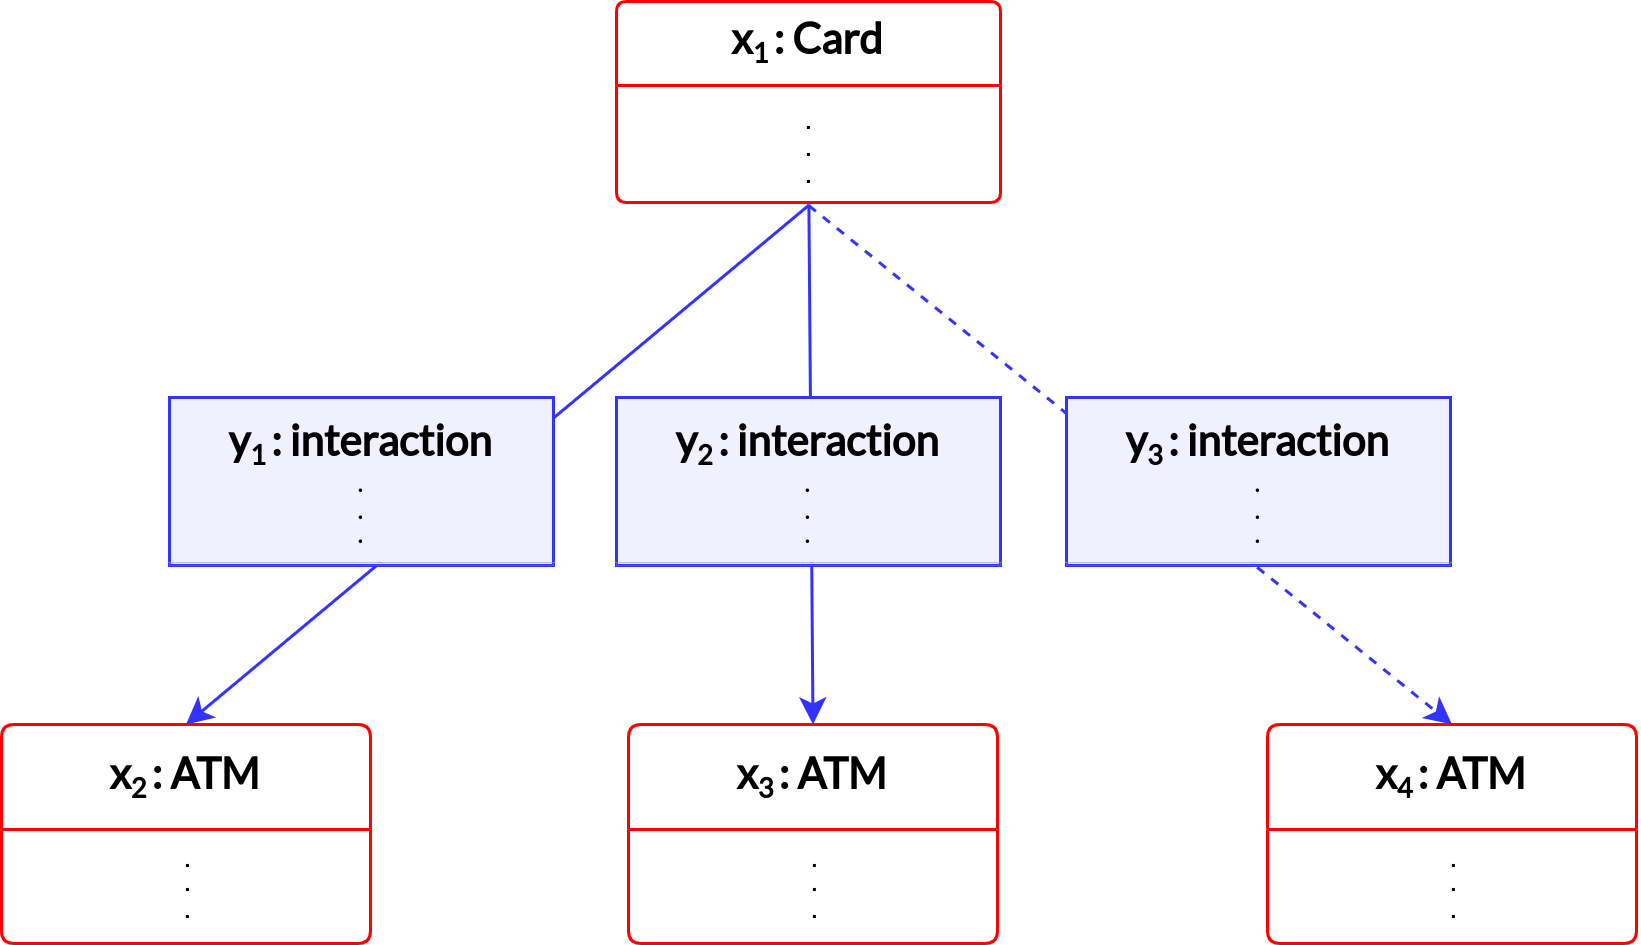
\includegraphics[scale = 0.7]{images/2-QueryModel/fp-I-demo-1.png}
  \caption{Subgraph $S$ of a card -- Fraud Pattern I}
  \label{img:fp-I-demo}
\end{figure}

Note that we can have that:
\begin{itemize}
    \item $F_I(y_2,y_3)$: We emit an alert of this anomalous scenario produced between the pair $(y_2,y_3)$. We could continue checking for anomalous scenarios between $y_3$ and previous edges of the subgraph. However, what we consider important for the bank system is to detect the occurrence of an anomalous scenario in a certain card. Therefore, we consider that, to achieve this, it is enough to emit a single alert of anomalous scenario on this card, and not many related with the same incoming transaction of the same card.
    \item $\neg F_I(y_2,y_3)$: We analyze whether it would be interesting or not to continue the checking with previous edges of the subgraph, based on assumptions on the fraud checking between previous edges. In particular we can have two cases:
    \begin{itemize}
        \item If $F_I(y_1,y_2)$: Having this it can happen that either $F_I(y_1,y_3)$ or $\neg F_I(y_1,y_3)$. In the case of $F_I(y_1,y_3)$, since $\neg F_I(y_2,y_3)$, we can infer that the anomalous scenario detected between $y_1$ and $y_3$ is a continuation of the same previous anomalous scenario detected between $y_1$ and $y_2$. Therefore, we can conclude that this does not constitute a new anomalous scenario that would require an alert.
        \item If $\neg F_I(y_1,y_2)$: It can be shown that \emph{by transitivity}, having \\
        $\neg F_I(y_1,y_2) \land \neg F_I(y_2,y_3)
        \implies \neg F_I(y_1,y_3)$. \\
        \textcolor{red}{TODO: Show a formal demostration of this case!}
    \end{itemize}
\end{itemize}

Therefore, we have seen that, it is enough to perform the checking between the pair formed by $e_{new}$ and the most recent edge of the subgraph $e_{last}$. $\square$

\textcolor{red}{TODO: Explain that we use this proof as a way to show that we do not need to store the full list of edges in the case of this fraud pattern (just the last edge). Maybe for others we need to store more / a list of edges.}


\textcolor{red}{\rule{\textwidth}{1pt}}
\textcolor{red}{TODO: Complete other aspects of the filter worker algorithmic workflow\\}
Others -- not so much related with the CheckFraud algorithm, but in general with the filter's algorithm --:
\begin{itemize}
    \item Save all the edges in the subgraph $S$, even though they are the reason of the creation of an anomalous scenario.
    \item Number of anomalous fraud scenarios that can be detected. Bounded by:
    $$\#TX\_ANOM \leq SCENARIOS \leq 2*\#TX\_ANOM$$
    \textcolor{red}{TODO: Poner dibujo y explicar mejor}
\end{itemize}

\textcolor{red}{\rule{\textwidth}{1pt}}

\begin{graysection}

\begin{comment}
\begin{algorithm}[H]
  \begin{algorithmic}[1]
  \STATE $e_i \gets \texttt{edgeChannel}$ \COMMENT{$e_i \in \texttt{Filter}_i$}
  \IF{$e_i.\texttt{type} = \texttt{interaction-start}$}
      \FOR{$e_s$ in $\texttt{Subgraph}_i$}
          \IF{$e_s.\texttt{id} \ne e_i.\texttt{id}\ \land$ \\
          \hspace{3.1em} $e_i.\texttt{start} - e_s.\texttt{end}  < T_{min}(e_i.\texttt{loc}, e_s.\texttt{loc})$}
              \STATE $\texttt{emitAlert}(e_i, e_s)$
          \ENDIF   
      \ENDFOR
  \ENDIF
  \end{algorithmic}
  \caption{FP1 check algorithm pseudocode}
\end{algorithm}


\paragraph{Possible Improvement}

Note that the checking of the ${FP}_1$ with respect to the new incoming edge $e_i$ is
performed against all the previous stored edges $e_s$ in the subgraph.\\ 
$\rightarrow$ With some kind of \textit{marking} strategy of the ${FP}_1$ in between 
the previous edges of the subgraph, in some of the cases, possibly, it will not be needed
to perform the checking of ${FP}_1$ of $e_i$ with respect of all the previous added
edges $e_s$: ${FP}_1(e_i, e_s)$

\begin{equation}
  \begin{cases}
    \nexists {FP}_1(e_i, e_s) \\
    \nexists {FP}_1(e_{s}, e_{s-1})
  \end{cases}\implies \nexists {FP}_1(e_i, e_{s-1}), \hspace{2em} \forall s, 1 < s < i\
\end{equation}

In this case, if somehow, it is marked that $\nexists {FP}_1(e_{s}, e_{s-1})$, and now 
we check that $\nexists {FP}_1(e_i, e_s)$, then due to a possible transitivity property,
we can show that $\nexists {FP}_1(e_i, e_{s-1}) \hspace{1em} \forall s, 1 < s < i$. 

% Drawing

\textcolor{red}{\rule{\textwidth}{1pt}}

\end{comment}


\subsection{Initial Tests}

In the following we describe the preliminar tests that were done to check the correct
expected behavior of the ${FP}_1$ algorithm.

\subsubsection{${FP}_1$ - Test 1}

\begin{figure}[H]
  \hspace*{-2cm} 
  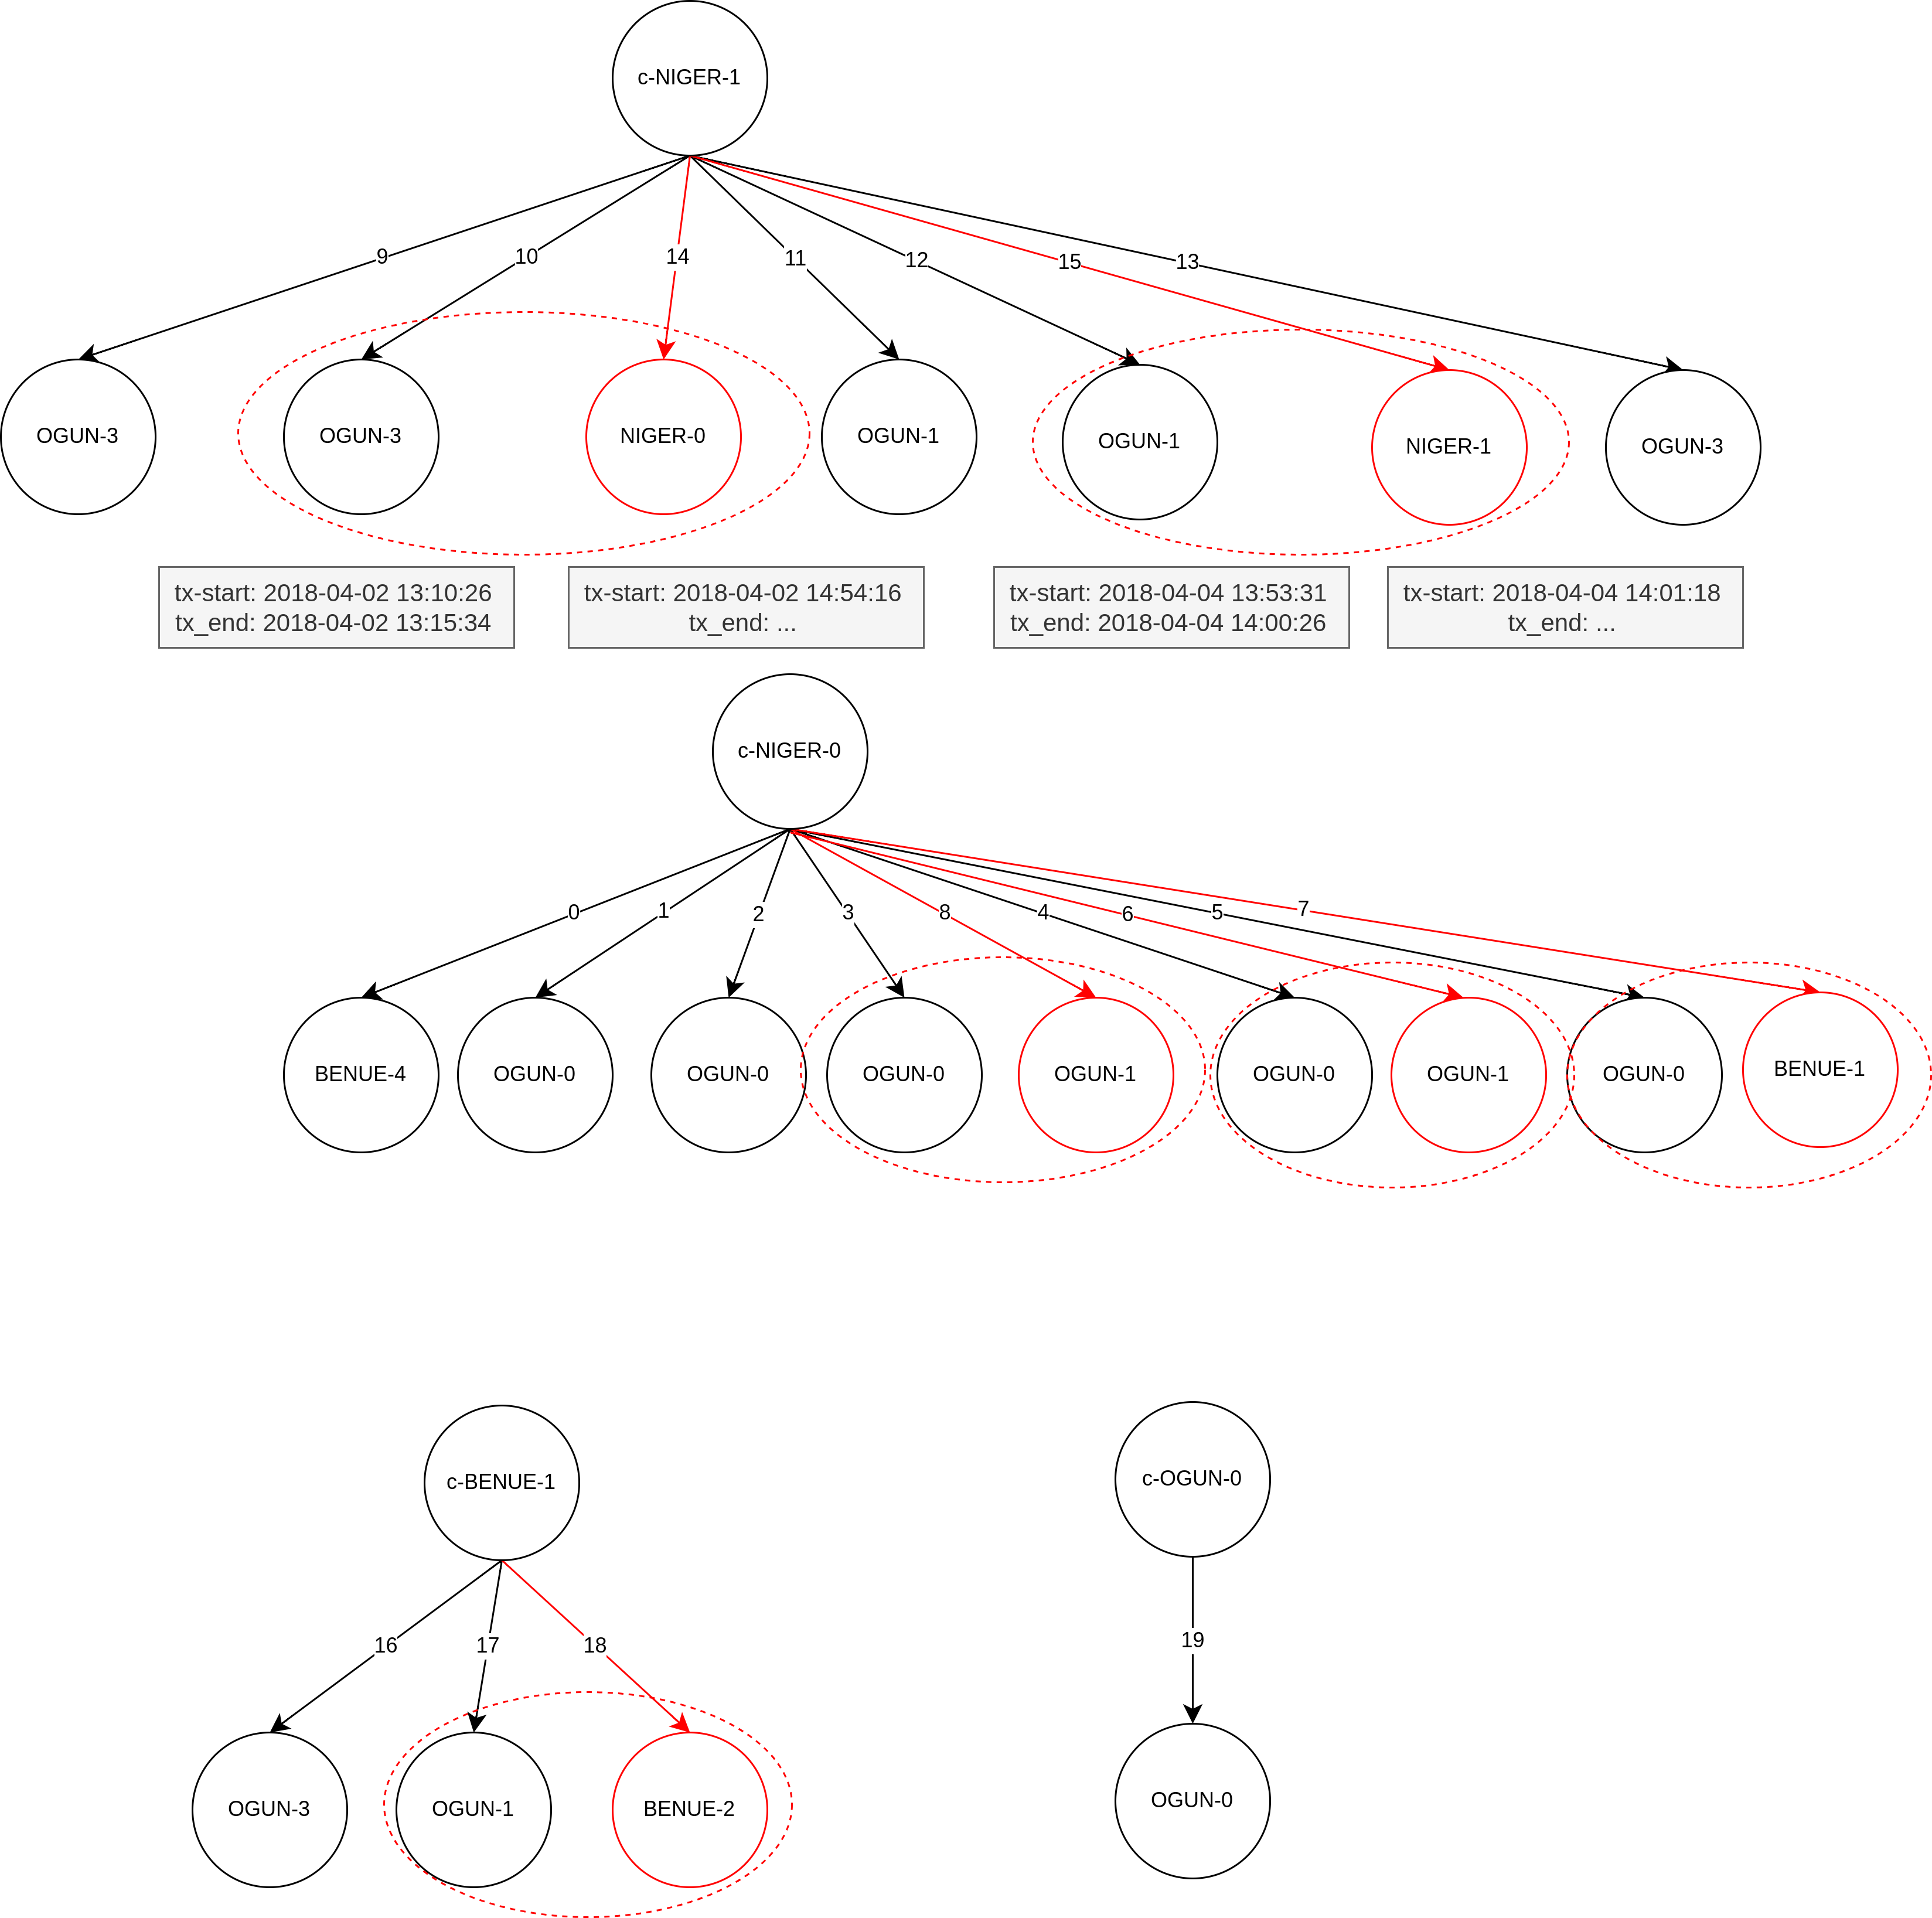
\includegraphics[scale=0.55]{images/2-QueryModel/FP1-test-1.png}
\end{figure}

\subsubsection{${FP}_1$ - Test 1.1}

\begin{figure}[H]
  \hspace*{-2cm} 
  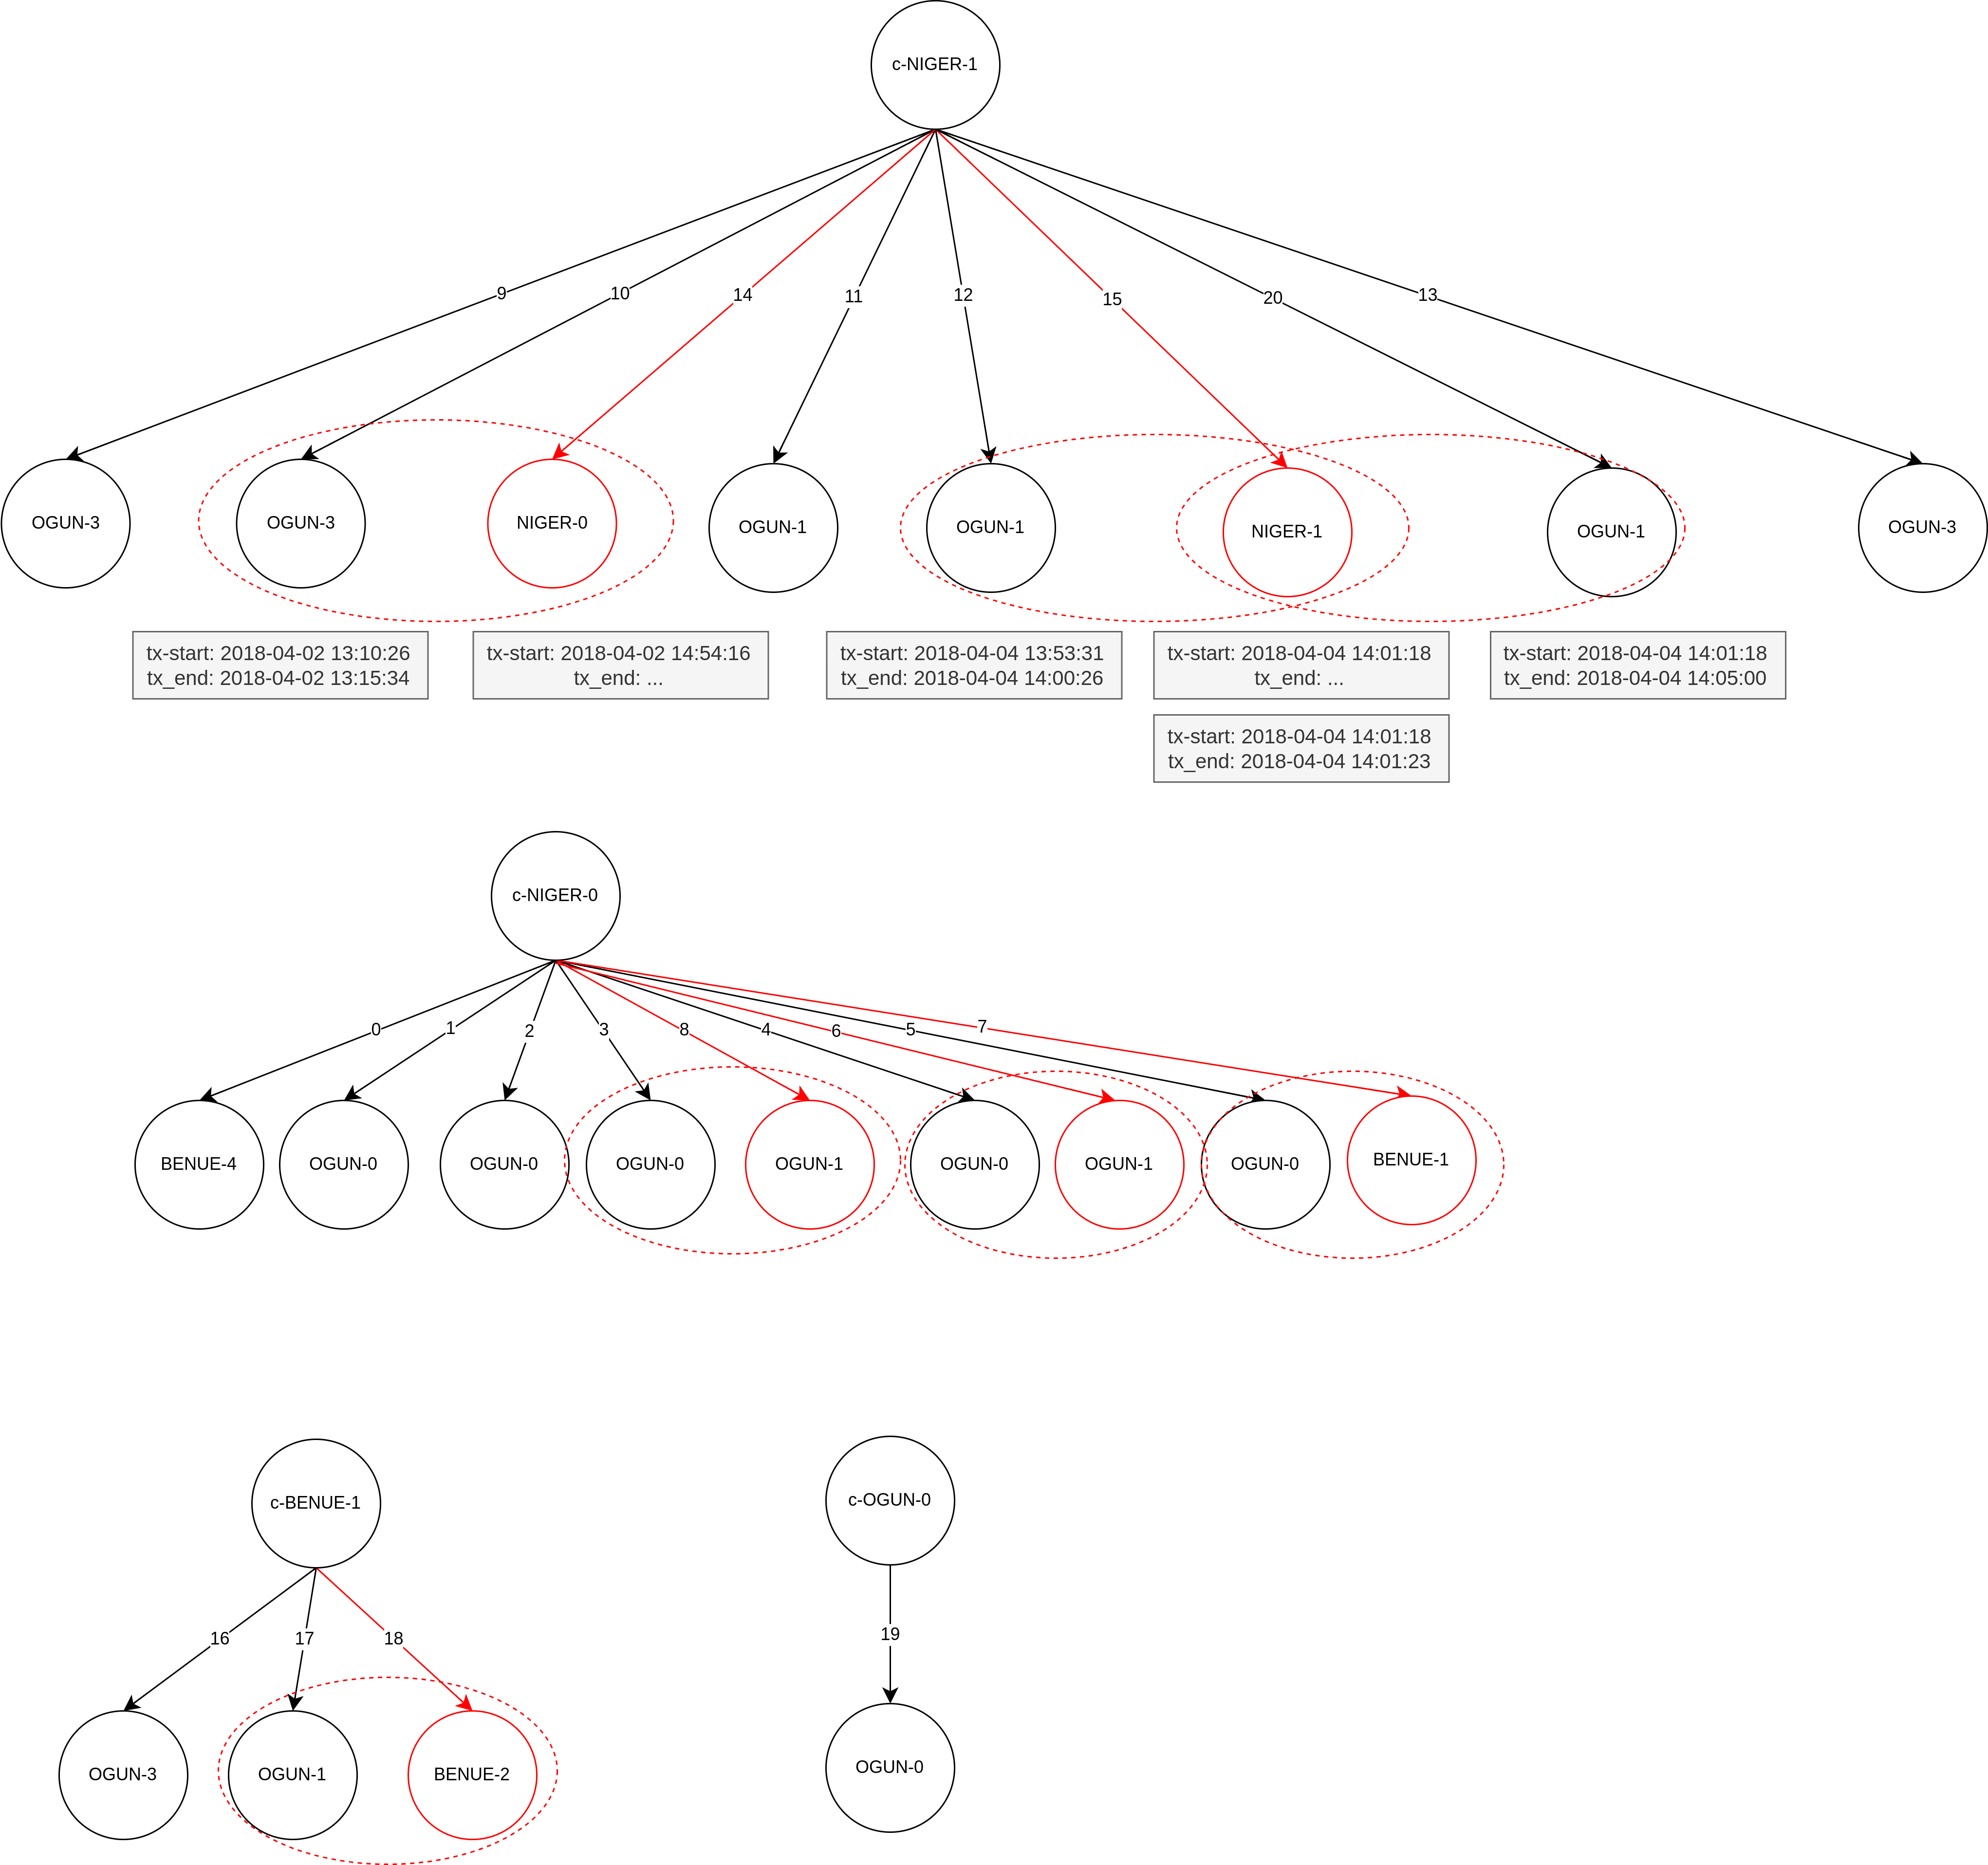
\includegraphics[scale=0.45]{images/2-QueryModel/FP1-test-1.1.png}
\end{figure}

\end{graysection}


